\documentclass[12pt, letterpaper,titlepage]{article}
\usepackage[margin=0.5in]{geometry}
\usepackage[utf8]{inputenc}
\usepackage{graphicx}
\usepackage{caption}
\usepackage{amsmath}
\usepackage{cite}
\graphicspath{ {figures/} }


\newcommand{\horrule}[1]{\rule{\linewidth}{#1}}
\title{	
\normalfont \normalsize 
\textsc{Oklahoma State University} \\ [25pt] 
\textsc{College of Engineering, Architecture and Technology} \\ [25pt]
\textsc{Department of Mechanical and Aerospace Engineering} \\ [25pt]
\horrule{0.5pt} \\[0.4cm] % Thin top horizontal rule
\huge  Mechatronics Design \\ 
\huge  Development of a Low Cost Open-Source Mobile Robotics Learning Platform\\
\horrule{0.5pt} \\[0.5cm] % Thick bottom horizontal rule
}



\author{Diego Alejadro Colón Serrano}
\date{May 7\textsuperscript{th}, 2020}

\begin{document}

\maketitle
\tableofcontents
\pagebreak

\section{Introduction}

	When looking for a mobile robotic platform to start in the hobby, it is quite daunting to select where to start. If you are completely new to programming and hardware design, a premade kit might seem like a good value proposition. The kit includes step-by-step instructions, all the parts required and there are many tutorials online on how to do things. Now, this option might be too simple for someone with more technical knowledge and is interested in mobile robotics and wants a platform to work with. Is there something that can fit the needs of both of them? Yes, there are but the prices of platforms that are accessible to newcomers but still relevant to experienced individuals are significant investments. For this reason, I set out to create a more budget-friendly mobile robotics platform that can be built and programmed by newcomers and expanded upon as they grow in the hobby. A platform that is simple to put together and work with but allows for possibilities past its original design. With that goal in mind, I designed a platform that achieves that which it's commercial competitors do while reducing the entrance price. \cite{DUMMY:1}

\section{Design}

\subsection{Design objectives}

	Before the design aspect of this project could take place, it was important to establish exactly what the design had to accomplish. For this project, the final concept must:

	\begin{enumerate}
		\item have a minimal cost.
		\item accessible to beginners and relevant to advanced users
		\item allow for additional expandability
		\item be able to be customized depending on the resources the user has available
		\item be a tool that allows the users to progress in the field towards more complex projects
	\end{enumerate}

\subsection{Benchmark}

	In order to complete this project a benchmark had to be established. A quick search on Amazon showed several different types of mobile robotics kits. These ranged from barebones kits that provided everything but a microcontroller such as (barebones) to kits that included everything required to get started such as (completes). The variety in entry level robotics kits is amazing and allows users to select something that fits their needs best. And although the complete kits do not offer as much flexibility as the barebones kits, users might favor a complete kit to avoid some of the complications that come with a barebones kit. 

	Currently the standard in mobile robotics platform for research appear to be Turtlebots. Turtlebots are small battery powered differential drive platforms controlled with a Raspberry Pi connected to a base computer. They are used to teach robotics classes at universities and as platforms for current robotics research. The software that is used to operate them is based on ROS (Robotics Operating System), an open-source project that has been the standard for robotics reserach and industrial applications. This is the standard for which the project will aim.

	The Turtlebot is currently in its third version and sells at a starting MSRP of 549.00 USD for the base model. The base model is equipped with: a Raspberry Pi 3, two encoded motors, 360 degree LiDAR sensor, 11.1V Li-Po battery, IMU unit and a low level control board to interract with the encoders and sensors. This combination of sensors, actuators and computation allows for a very versitile platform on which many different aspects of mobile robotics can be investigated and explored.

\subsection{Mechanical Design}

	For the mechanical design of the project it was assumed that the user has access to a 3D printer which although not necessary for the project, it makes the fabrication simpler. With this in mind, it was decided to make the structure as simple and printer-friendly as possible. The structure consists of several stacked plates that are held together by standoffs and 3mm bolts. The figure below shows what the plates look like.

	\begin{figure}[h]
	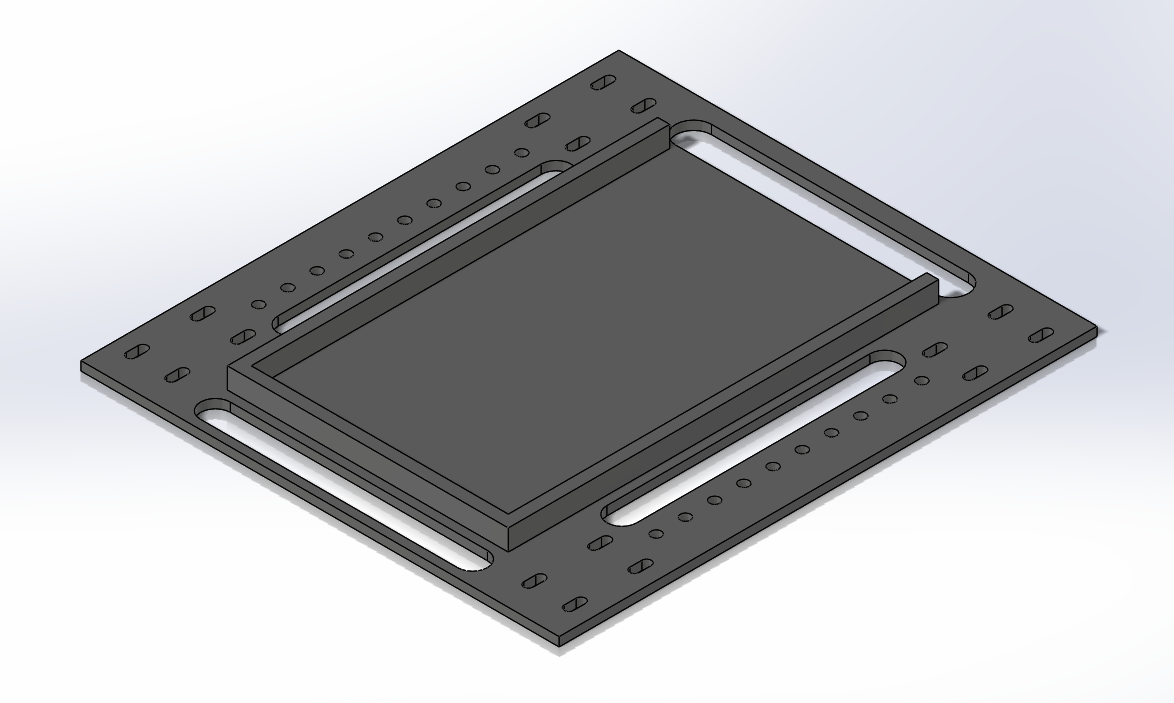
\includegraphics[width=0.5\textwidth]{plate.png}
	\centering
	\caption{Plates on which the structure is based on}
	\end{figure}

	Each plate has: a group of 4 slots on each corner on to which the motors are mounted, four large slots for cables to be guided through, two rows of holes to secure adjacent plates, and a cavity for the battery to be placed in. This design allows for the user to 3D print as many plates as they want and expand their robot.
	
	\begin{figure}[h]
		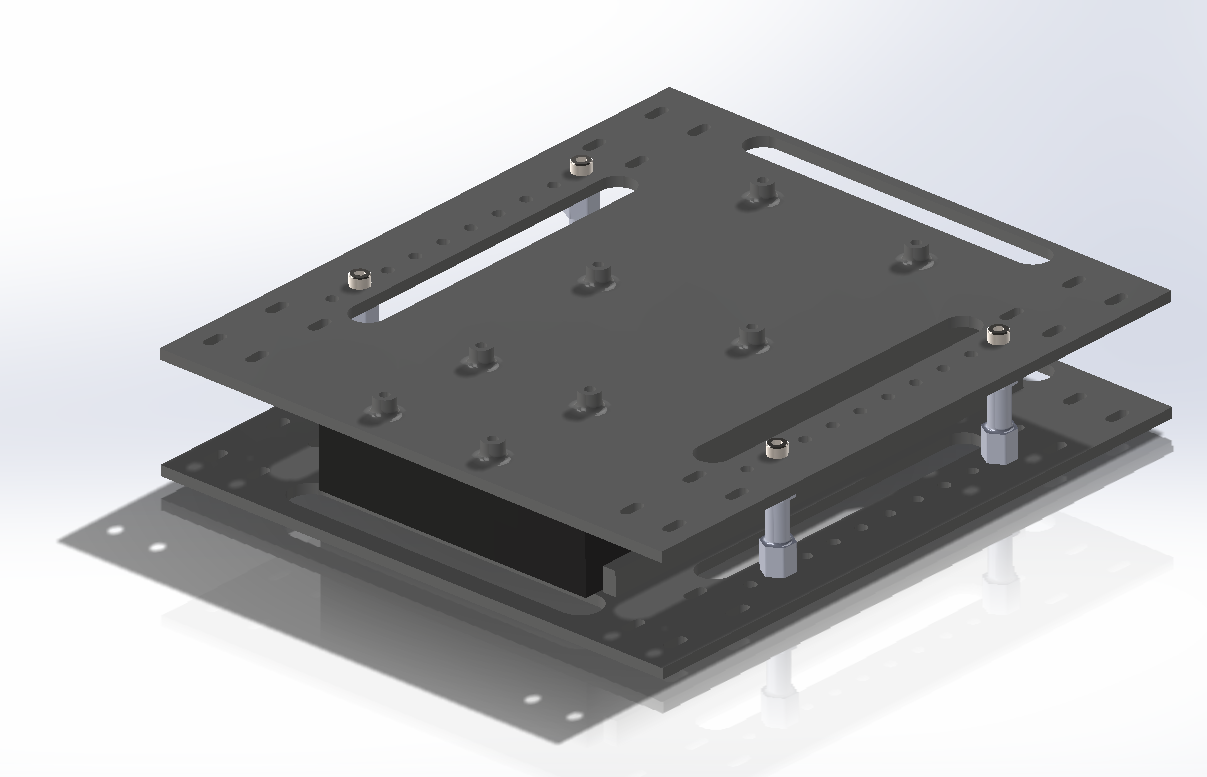
\includegraphics[width=0.5\textwidth]{plate_assembly.png}
		\centering
		\caption{Plate and battery assembly}
	\end{figure}

\subsection{Electrical Design}

	The electrical design was made as simple as possible to not intimidate newcomers. This meant that soldering was not considered, and that the majority of the wiring had to be "plug and play" as opposed to having to splice wires together, worry about battery protection circuits, etc. The electrical design consists of a Raspberry Pi 4 connected to a  DFROBOT IO Expansion Hat which simplifies the connections between the the Raspberry Pi and the rest of the hardware. This is powered by a 12V Lithium Ion battery pack whose voltage is reduced to 5 volts through a buck converter. The IO Expansion Hat has four PWM ports, two of which are connected to the H-Bridge to drive the motors, and many digital pins, four of which are connected to the H-Bridge to determine direction of the motors.

\subsection{Software Design}

	The software has to be simple for a newcomer to pick it up while being relevant to the current industrial and research in mobile robotics. This led to the the robot's initial software to be based around ROS. ROS provides the ability to program in different languages, mainly C++ and Python. This allows for newcomers to learn by starting with Python given its simplicity and work their way up to more advanced programs in C++. ROS also has a great community base with resources and tutorials to learn how it operates in both C++ and Python. 

	Apart from this, the way that the user structures the software is completely up to them, but for the purposes of this project I created an example in which through a joystick, velocity commands are sent to the robot and it returns visual feebback from a camera. All of the code was written in Python without using prewritten ROS packages and is available on my Github (https://github.com/dacsgb/Mechatronics-Project.git).

\section{Validation}
	To validate the that the the platform achieved its goal of lowering the financial barrier for people to have access to a mobile robotics platform, the cost of the project was compared to the MSRP of the Turtlebot. If the platform cost less than the MSRP of the Turtlebot, while maintaining similar fuctionalities, the project was successful.

\subsection{Procedures}

	The general procedures for the project were as follow:

	\begin{itemize}
		\item Identify minimum requirements for the platform based on the Turtlebot 3
		\item Model platform in Solidworks
		\item Cost design based on prices on Amazon
		\item Build prototype with parts available
		\item Demonstrate functionality with example code
	\end{itemize}




\section{Results}
	Demonstrate your mechatronc system (simulator or experiment). Provide a link to your demonstration. Collect and present necessary dtat to prove the effectiveness of your design

\section{Discussion}

\section{Conclusions}

\section{Recommendations}

\bibliographystyle{IEEEtran}
\bibliography{research}

\end{document}